% ====================================
% Zusammenfassung, Fazit und Ausblick
% ====================================

\chapter{Fazit und Ausblick}

Insgesamt l�sst sich feststellen, dass die Implementation f�r viele Gitterpunkte bei allen vorgestellten Beispielen realit�tsnahe Ergebnisse liefert. Bei einer kleineren Gitterweite erhalte ich nicht das Ergebnis, was ich erwarte, wie z.B. bei \ref{fig:riss_ganz_mitte_10_gitter.riss} und \ref{fig:riss_ganz_mitte_10_gitter.gebiet}. Hier rei�t das Material am Rand und nicht in der Mitte. Das selbe Problem l�sst sich auch bei anderen Beispielen finden, die ich hier aufgrund des Umfangs nicht pr�sentieren kann. Eine m�gliche Erkl�rung ist, dass der Riss sehr gro� im Vergleich zu dem Material ist und jegliche Fortsetzung des Risses schon dazu f�hrt, dass das Material auch am Rand gerissen wird. 

\begin{figure}[!bth]
	\centering	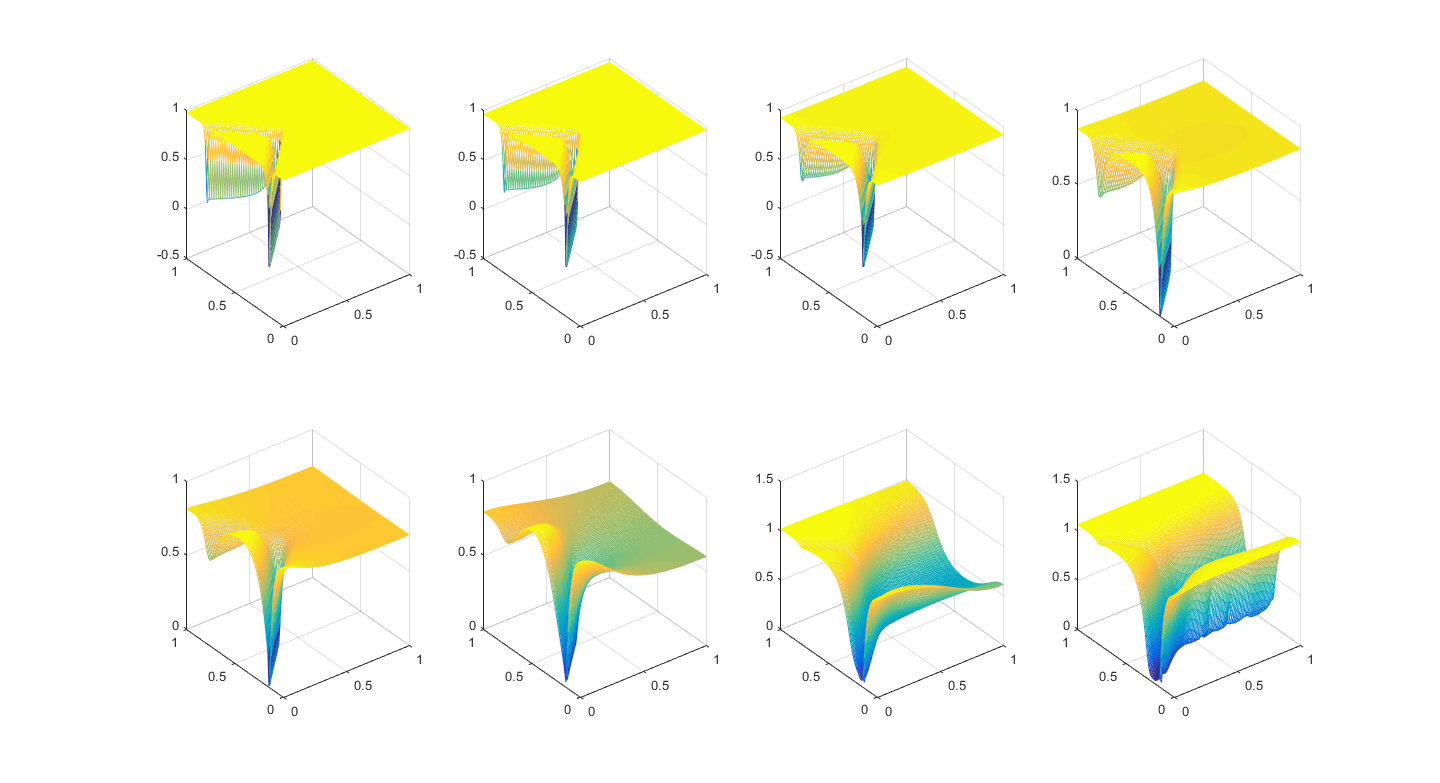
\includegraphics[scale=0.40]{images/optimazation/02_2_rissAnEinerSeite_100Gitter_u0Konstant.png}
	\caption{Darstellung des Risses  bei konstantem $u_0$, zwei kleinen Riss an einem Rand und $100x100$ Gitterpunkten}
	\label{fig:2riss_eineSeite_100_gitter.riss}
\end{figure}

Ein anderes, nicht funktionierendes Beispiel zeigt die Modellierung von zwei Rissen, die in einem Material auf der gleichen Seite sind und aufeinander zu laufen. Ein Riss verschwindet komplett bei vielen Iterationen, wie in Abbildung \ref{fig:2riss_eineSeite_100_gitter.riss} dargestellt. Dies d�rfte nicht sein, da, wenn das Material einmal gerissen ist, der Riss immer dort bleiben sollte. Weiterf�hrend k�nnte betrachtet werden, warum dieser Riss verschwindet. Vielleicht ist dies ein Problem der Modellierung.

Betrachten wir die Laufzeit der Implementation. Diese liegt bei $O(n^2)$, wobei $n$ die Breite bzw. H�he des Gitters ist. Dieses ist in \ref{fig:laufzeit} zu sehen. Eigentlich sollte es in $O(n)$ m�glich sein, das Problem zu implementieren, da nur Matrizen aufgestellt werden und mehrere Matrixmultiplikationen mit Sparse-Matrizen stattfinden, die sehr effizient sind. Beim genaueren Betrachten des Codes f�llt auf, dass meine Implementation sehr viel Zeit bei dem erstellen der Matrizen braucht. Dieses k�nnte vermutlich sehr viel schneller gehen. 

 \begin{figure}[!htb]
 	\centering	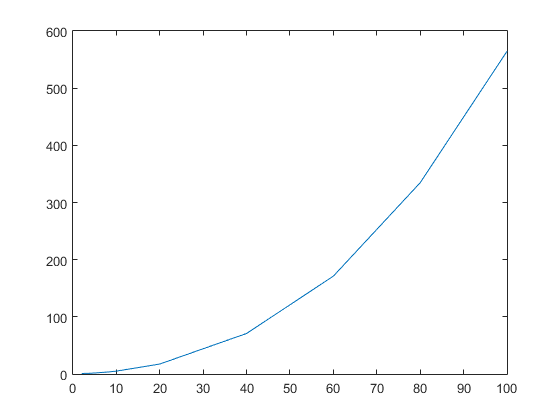
\includegraphics[scale=0.42]{images/laufzeit.png}
 	\caption{Laufzeit der Implemention. Auf der x-Achse ist die Gitterweite, auf der y-Achse die Zeit in Sekunden angegeben}
 	\label{fig:laufzeit}
 \end{figure}

In der analytischen Betrachtung k�nnte man untersuchen, ob weniger Voraussetzungen an $u_0$ und $v_0$ gestellt werden m�ssen. Stetigkeit von $u_0$ sollte ausreichend sein, ist aber auch notwendig. In der Praxis kann man Material nicht unstetig einspannen.  

Eine wichtige Untersuchung w�re die Konvergenz der Newton Methode. Diese zu beweisen erweist sich als sehr schwierig, da nicht klar ist, ob die Regularit�tsannahme erf�llt ist. Im Diskreten konvergiert die Methode f�r alle untersuchten Beispiele, was nat�rlich keine Aussage dar�ber trifft, ob sie auch im analytischen Sinn konvergiert. 

